\subsection{Etapa impulsora}

Identificamos la etapa impulsora en el diagrama del amplificador multietapas, la cual es la que contiene al  transistor $Q_3$. Dicha etapa se muestra en la ilustración \ref{ilus:met-etapa-impulsora}.

\begin{ilustracion}[ht]
    \centering
    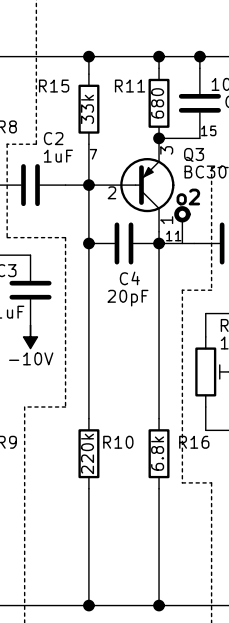
\includegraphics[width=0.23\textwidth]{src/images/p3/etapa-impulsora.png}
    \caption{Etapa impulsora del amplificador}
    \label{ilus:met-etapa-impulsora}
\end{ilustracion}

aplicamos thevenim de manera que:

$$R_{th}= R15 || R10$$

$$R_{th}=29 k\Omega$$

$$V_{th} = \frac{R15}{R15 + R10} (V_{cc} - V_{ee})$$

$$V_{th} = 2.61 V $$

Aplicando LVK en la malla del emisor:

$$V_{th} - V_{be} = R11 \beta I_{b} + R_{th}I_b$$

$$ Ib = \frac{V_{th} - V_{be}}{R11\beta + R_{th}}$$

usando un $\beta = 230$

$$ I_b = 10.03 \mu A$$

$$Ic = \beta I_b$$

$$I_c = 2.37 mA$$

Aplicando LVK:

$$V_{ce} = V_{cc} - V_{ee} - I_eR11 - I_cR16$$

$$ V_{ce} = 2.27 V$$

La tabla \ref{tab:etapa-impulsora-puntos-estaticos} presenta los puntos estáticos de operación en la etapa impulsora.

\begin{table}[ht]
    \centering
    \begin{tabular}{|c|c|c|}
        \hline
        Transistor & \textbf{$I_c$} & \textbf{$V_{ce}$} \\
        \hline
        $Q_3$ & $2.37 mA$ & $2.27 V$ \\
        \hline
    \end{tabular}
    \caption{Puntos estáticos de operación en la etapa impulsora}
    \label{tab:etapa-impulsora-puntos-estaticos}
\end{table}

La ilustración \ref{ilus:sim-etapa-impulsora-puntos-estaticos} muestra la simulación de los puntos estáticos de operación en la etapa impulsora.

\begin{ilustracion}[ht]
    \centering
    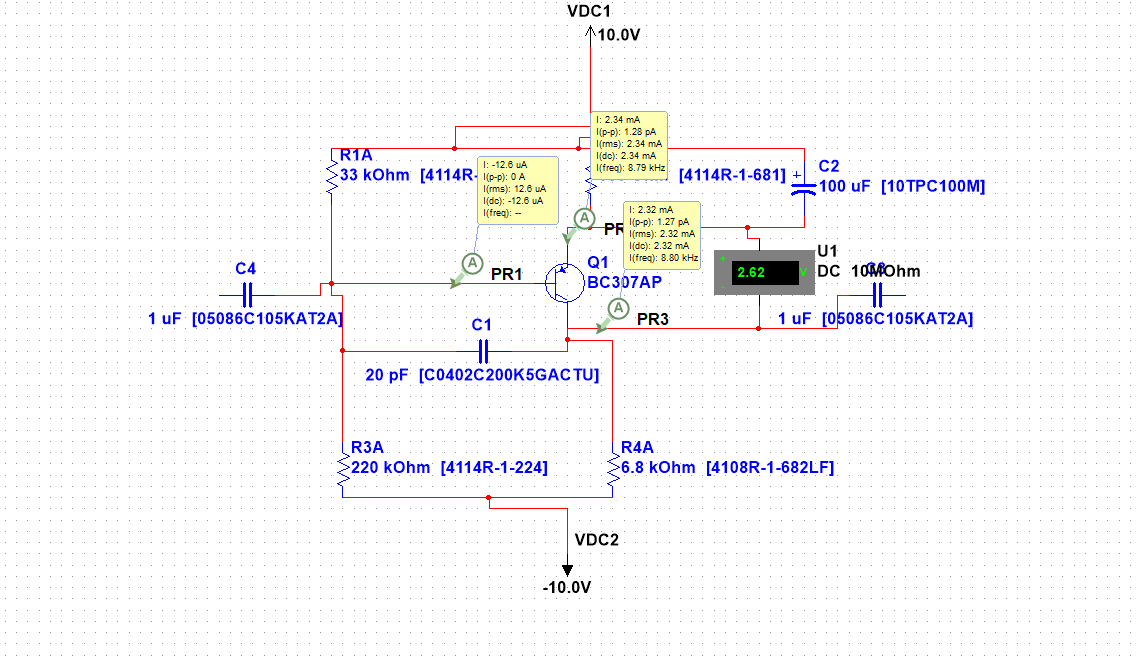
\includegraphics[width=0.9\textwidth]{src/images/p3/ punto-estatico-etapa-impulsora.png}
    \caption{Simulación puntos estáticos etapa impulsora}
    \label{ilus:sim-etapa-impulsora-puntos-estaticos}
\end{ilustracion}

Haciendo el analisis AC, tenemos 
$$gm = \frac{I_{c}}{V_t} = 0.09$$

$$R_{\pi} = \frac{\beta}{gm} = 2523$$

$$R_o = \frac{V_A}{I_c} = \frac{100V}{2.37mA} = 42,20k\Omega$$

\begin{table}[ht]
    \centering
    \begin{tabular}{|c|c|c|c|}
        \hline
        Transistor & $R_\pi$ & $gm$ & $R_o$ \\
        \hline
        $Q_3$ & $2.52 k\Omega$ & $0.09S$ & $42.20k\Omega$ \\
        \hline
    \end{tabular}
    \caption{Parámetros dinámicos de la etapa impulsora}
    \label{tab:met-etapa-impulsora-parametros-dinamicos}
\end{table}


La impedancia de entrada es:

$$Z_i = R15 || R10 || r_\pi $$
$$z_i = 2.31 k \Omega $$

Para calcular la impedancia de salida, aplicamos la ecuación:

$$ Z_o = Z_{cc} \parallel r_{16}$$

pero, como $Z_{ccQ1} >> r_3$ entonces:

$$ Z_o = r_{16} $$
$$ Z_o = 6.8k\Omega$$

para calcular la ganancia tenemos:

$$A = \frac{gmr_\pi R16}{r_\pi} = 619.90$$

La ilustración \ref{ilus:sim-etapa-impulsora-ganancia} muestra la simulación de la ganancia en la etapa impulsora.

\begin{ilustracion}[ht]
    \centering
    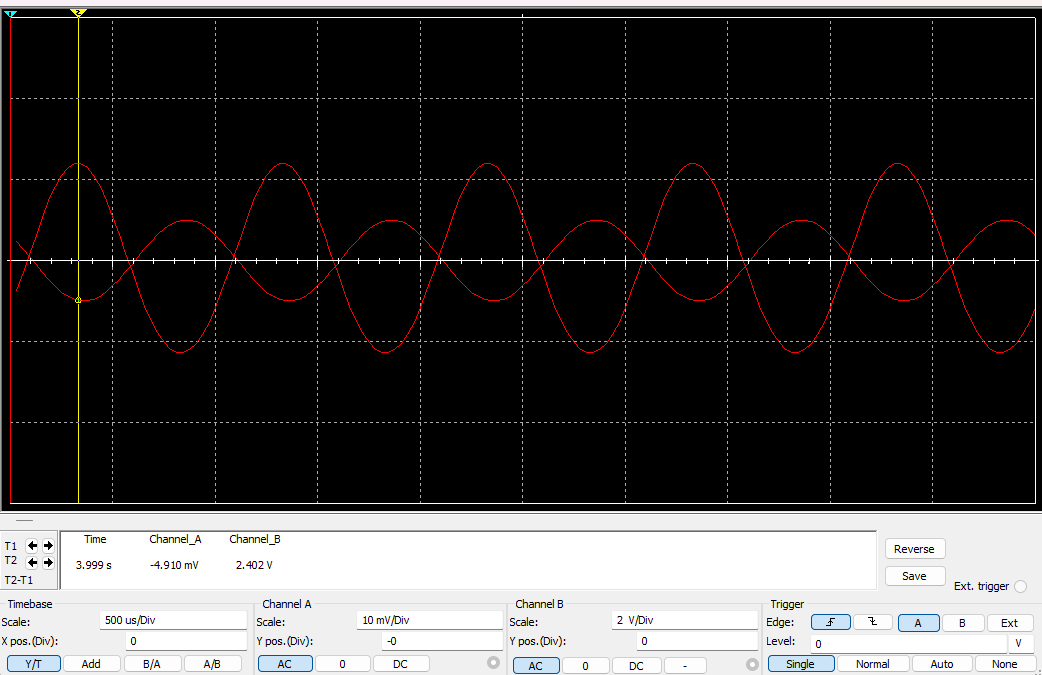
\includegraphics[width=0.9\textwidth]{src/images/p3/etapa-impulsora-ganancia.png}
    \caption{Simulación ganancia etapa impulsora}
    \label{ilus:sim-etapa-impulsora-ganancia}
\end{ilustracion}

La tabla \ref{tab:met-etapa-impulsora-parametros-dinamicos} presenta el modelo dinamico de la etapa impulsora.

\begin{table}[ht]
    \centering
    \begin{tabular}{|c|c|}
        \hline
        parámetro & valor  \\
        \hline
        $Z_i$ & $2.31k\Omega$ \\
        \hline
        $Z_o$ & $6.8k\Omega$ \\
        \hline
        $A$ & $619.90$ \\
        \hline
    \end{tabular}
    \caption{Modelo dinámico de la etapa impulsora}
    \label{tab:met-etapa-impulsora-modelo-dinamico}
\end{table}


\subsection{Amplificador multietapas}

Los puntos de de operación del amplificador multietapas son todos aquellos que se calcularon para las etapas individuales. Mientras que en el modelo dinámico para las impedancias de entrada se utilizan las de la etapa diferencial tanto en modo común como en modo diferencial. Por otro lado, la impedancia de salida es la misma que la de la etapa de potencia.


Para encontrar la ganancia en el modo diferencial se analiza analiza todo el circuito, puediendo dividir la expresión en distintas partes de forma que:

$$ A_d = A_1 A_2 A_3 $$

donde $A_1$ es la ganancia desde la etapa diferencial, que viene dada por:

$$ A_1 = \frac{-gmr_{\pi1} R_3 \parallel r_{15} \parallel r_{10} \parallel r_{\pi3}}{r_{\pi1} + (1+ gmr_{\pi_1})(r_5 + \frac{r_{\pi2}}{1 + gmr_{\pi2}})}$$

 $$A_1 = - 1.03 $$

 $A_2$ es la ganancia vista desde la etapa impulsora, que viene dada por:

 $$ A_2 = \frac{-gmr_{\pi3} R_{16} \parallel r_{17} \parallel r_{12} \parallel [r_{\pi5} + (1 + gmr_{\pi 5})(r_{13} + r_l)]}{r_{\pi 3}}$$

 $$A_2 =- 383.52 $$

 $A_3$ es la ganancia vista desde la etapa potencia, que viene dada por:

 $$ A_3 = \frac{(1 + gmr_{\pi5})(r_{13} + r_l)r_l}{[r_{\pi 5} + (1 + gmr\pi5)(r_{13} + r_l)](r_{13} + r_l)}$$

 $$A_3 = 0.96 $$

Por lo que la ganancia diferencial es: 

$$ A_d = 1.03 \times 383.52 \times 0.96 = 1.03 \times 383.52 \times 0.96 = 379.22 $$

La tabla \ref{tab:met-amp-multietapas-mod-diferencial} presenta el modelo dinámico del amplificador multietapas en modo diferencial.

\begin{table}[ht]
    \centering
    \begin{tabular}{|c|c|}
        \hline
        parámetro & valor  \\
        \hline
        $Z_i$ & $43,99k\Omega$ \\
        \hline
        $Z_o$ & $132\Omega$ \\
        \hline
        $A$ & $379.22$ \\
        \hline
    \end{tabular}
    \caption{Modelo dinámico amplificador multietapas en modo diferencial}
    \label{tab:met-amp-multietapas-mod-diferencial}
\end{table}

La ilustración \ref{ilus:sim-amp-multietapas-mod-diferencial} muestra la simulación del amplificador multietapas en modo diferencial.

\begin{ilustracion}[ht]
    \centering
    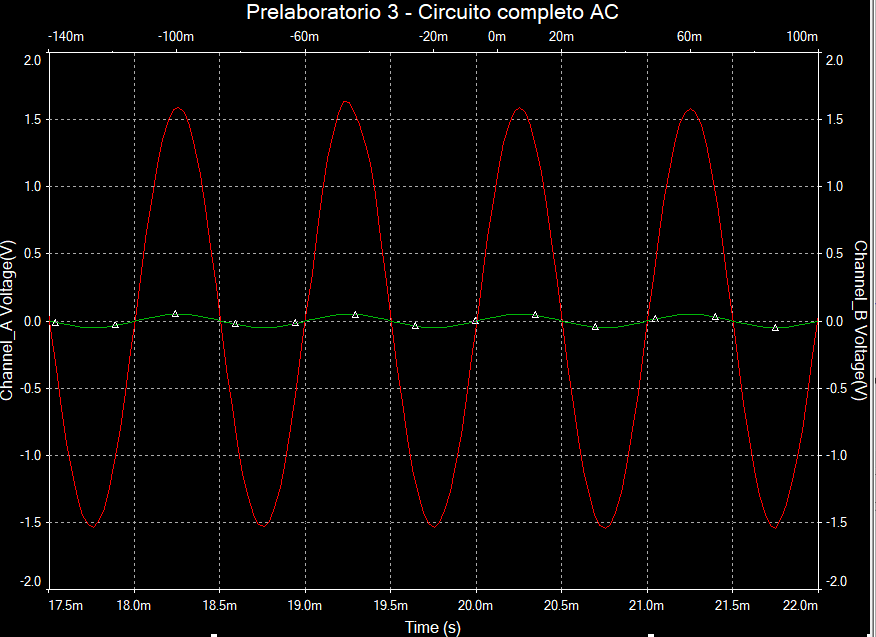
\includegraphics[width=0.9\textwidth]{src/images/p3/multietapa-modo-diff-ganancia.png}
    \caption{Simulación amplificador multietapas en modo diferencial}
    \label{ilus:sim-amp-multietapas-mod-diferencial} 
\end{ilustracion}

Para encontrar el valor de la ganancia en el modo común se utiliza la misma fórmula que en el modo diferencial pero se reemplaza el valor de $A_1$ por:

$$ A_1 = \frac{-gmr_{\pi1} R_3 \parallel r_{15} \parallel r_{10} \parallel r_{\pi3}}{r_{\pi1} + (1+ gmr_{\pi_1})r_4}$$

$$ A_1 = -0.11 $$

Por lo tanto, la ganancia en modo común es:

$$ A_c = A_1 A_2 A_3 = 0.11 \times 383.52 \times 0.96 = 0.11 \times 383.52 \times 0.96 = 40.05 $$

La tabla \ref{tab:met-amp-multietapas-mod-comun} presenta el modelo dinámico del amplificador multietapas en modo común.

\begin{table}[ht]
    \centering
    \begin{tabular}{|c|c|}
        \hline
        parámetro & valor  \\
        \hline
        $Z_i$ & $24.5k\Omega$ \\
        \hline
        $Z_o$ & $132\Omega$ \\
        \hline
        $A$ & $40.05$ \\
        \hline
    \end{tabular}
    \caption{Modelo dinámico amplificador multietapas en modo común}
    \label{tab:met-amp-multietapas-mod-comun}
\end{table}

La ilustración \ref{ilus:sim-amp-multietapas-mod-comun} muestra la simulación del amplificador multietapas en modo común.

\begin{ilustracion}[ht]
    \centering
    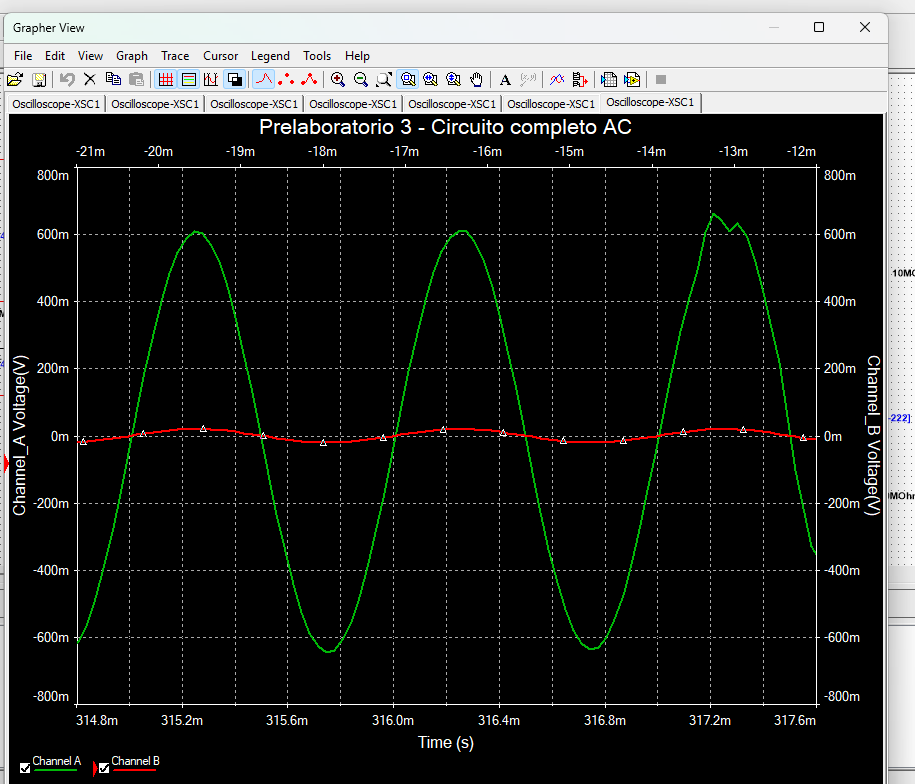
\includegraphics[width=0.9\textwidth]{src/images/p3/multietapa-modo-comun-ganancia.png}
    \caption{Simulación amplificador multietapas en modo común}
    \label{ilus:sim-amp-multietapas-mod-comun}
\end{ilustracion}
